\begin{enumerate}[label=(\roman*)]
    \item 

The data are generated according to
\[
y_i = \beta_1 + \beta_2 x_{i2} + \beta_3 x_{i3} + \beta_4 x_{i4} + \varepsilon_i,
\]
where $\varepsilon_i \sim N(0,\sigma^2)$ and $n = 35$.  

The true parameter values in the $dgp$ are $\beta_1 = 10$ and $\beta_2 = \beta_3 = \beta_4 = 0.5$. The model is estimated by Ordinary Least Squares (OLS):
\[
\hat{\beta} = (X'X)^{-1} X'y,
\]
where $X$ is the $n \times K$ matrix of observations on the constant and regressors, and $y$ is the $n \times 1$ vector of dependent-variable observations. Under the Gauss–Markov assumptions and normal disturbances, the statistic
\[
t_k = \frac{\hat{\beta}_k - \beta_k}{se(\hat{\beta}_k)} \sim t(n-K),
\]
follows a Student-t distribution in finite samples, where
\[
se(\hat{\beta}_k) = \sqrt{\hat{\sigma}^2[(X'X)^{-1}]_{kk}}, \qquad
\hat{\sigma}^2 = \frac{\hat{\varepsilon}'\hat{\varepsilon}}{n-K}.
\]
Hence, the 95\% confidence interval for each parameter is
\[
\hat{\beta}_k \pm t_{0.975}(n-K)\,se(\hat{\beta}_k).
\]

\noindent The estimation was carried out in \texttt{R} using:
\begin{verbatim}
model <- lm(y ~ x2 + x3 + x4, data = data33)
summary(model)
confint(model, level = 0.95)
\end{verbatim}

\begin{table}[H]
\centering
\caption{OLS estimates and 95\% confidence intervals.}
\begin{tabular}{lccccc}
\hline
Variable & Estimate & Std.\ Error & t value & Pr(>|t|) & 95\% CI \\ 
\hline
(Intercept) & 7.9365 & 1.6427 & 4.832 & 0.00003 & [4.586 , 11.287] \\
$x_{2}$ & 0.5953 & 0.0747 & 7.970 & 0.00000 & [0.443 , 0.748] \\
$x_{3}$ & 0.2996 & 0.5264 & 0.569 & 0.573 & [-0.774 , 1.373] \\
$x_{4}$ & 0.7819 & 0.5278 & 1.481 & 0.149 & [-0.294 , 1.858] \\
\hline
\multicolumn{6}{l}{\footnotesize Residual standard error: 3.508 (df = 31)}\\
\multicolumn{6}{l}{\footnotesize $R^2 = 0.8856$, Adjusted $R^2 = 0.8745$, F-statistic = 79.95, p-value = $1.10\times10^{-14}$}\\
\end{tabular}
\end{table}

\noindent
The estimate of $\hat{\beta}_2 = 0.595$ is positive and statistically significant, consistent with the true value $\beta_2 = 0.5$.  
Coefficients $\hat{\beta}_3$ and $\hat{\beta}_4$ have the expected positive signs but are imprecisely estimated, with wide confidence intervals that include zero.  
This is due to the high correlation between $x_{3}$ and $x_{4}$ ($\operatorname{corr}(x_{3},x_{4}) \approx 0.9$), which increases the sampling variance of their estimators:
\[
\operatorname{var}(\hat{\beta}_k \,|\, X) = \sigma^2 [(X'X)^{-1}]_{kk}.
\]
The model exhibits a high $R^2 = 0.8856$, indicating a good overall fit, although inference on $x_{3}$ and $x_{4}$ is unreliable because of collinearity.

\item
Under the classical linear model assumptions, the OLS estimator satisfies
\[
\hat{\beta} \,|\, X \sim N\!\big(\beta,\, \sigma^2 (X'X)^{-1}\big).
\]

For the parameters $\beta_3$ and $\beta_4$, the joint 95\% confidence region is defined as the set of all points $(\beta_3, \beta_4)$ that satisfy
\[
(\hat{\beta} - \beta)' 
\Big[\hat{\sigma}^2 (X'X)^{-1}\Big]^{-1}
(\hat{\beta} - \beta)
\le \chi^2_{2}(0.95),
\]
where $\chi^2_{2}(0.95)$ denotes the 95th percentile of the chi-squared distribution with two degrees of freedom.  
This inequality describes an ellipse centered at $(\hat{\beta}_3, \hat{\beta}_4)$, since $(\hat{\beta}_3, \hat{\beta}_4)$ are jointly normally distributed.

\medskip
\noindent
The 95\% confidence region was obtained in \texttt{R} using the \texttt{confidenceEllipse()} function from the \texttt{car} package:

\begin{verbatim}
library(car)
confidenceEllipse(model, c("x3", "x4"), levels = 0.95, lwd = 2)
abline(v = confint(model)["x3", ], lty = 2)
abline(h = confint(model)["x4", ], lty = 2)
points(coef(model)["x3"], coef(model)["x4"], pch = 19)
title("95% Confidence Ellipse for (β3, β4)")
\end{verbatim}

\begin{figure}[H]
\centering
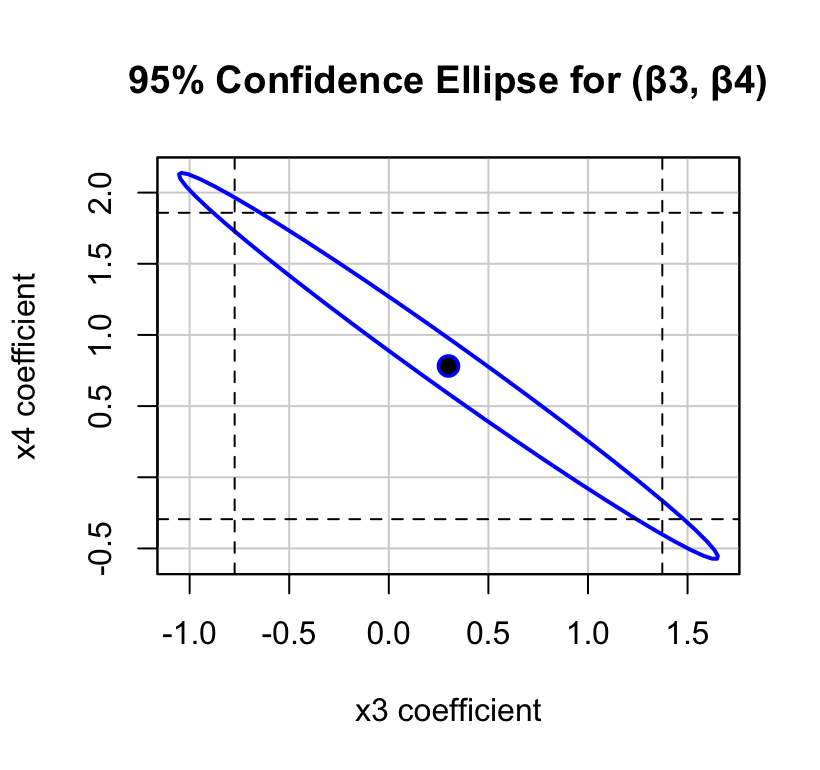
\includegraphics[width=0.65\textwidth]{fig/1aii.png}
\caption{95\% joint confidence region for $(\beta_3 \text{ and } \beta_4)$ (blue ellipse) with marginal confidence intervals (dashed lines).}
\label{fig:ellipse}
\end{figure}

\item
The ellipse in Figure~\ref{fig:ellipse} represents the joint 95\% confidence region for $(\beta_3, \beta_4)$.  
The dashed vertical and horizontal lines correspond to the marginal 95\% confidence intervals for each parameter, and the black point marks the OLS estimates $(\hat{\beta}_3, \hat{\beta}_4)$.  
The ellipse is elongated and negatively sloped, reflecting the negative correlation between $\hat{\beta}_3$ and $\hat{\beta}_4$, caused by the strong collinearity between $x_3$ and $x_4$.  

\medskip
\noindent

Since the origin $(0, 0)$ does not lie within the ellipse, the joint null hypothesis
\[
H_0 : \beta_3 = \beta_4 = 0
\]
can be rejected at the 5\% significance level. In comparison, we cannot reject the hypothesis that $\beta_3 = 0$ or $\beta_4=0$ separately. 


\item 
The figure illustrates the difference between testing the significance of regressors separately and jointly.  

\medskip
\noindent
\textbf{Separate tests:}  
Testing each coefficient individually (e.g., $H_0 : \beta_3 = 0$ and $H_0 : \beta_4 = 0$) relies on the marginal confidence intervals for $\beta_3$ and $\beta_4$, represented by the vertical and horizontal dashed lines in the figure. Each test ignores the covariance between the two estimates. Since both intervals include zero, we cannot reject either of the null hypothesis. 

\medskip
\noindent
\textbf{Joint test:}  
The ellipse represents the set of $(\beta_3, \beta_4)$ values that are jointly consistent with the data at the 5\% significance level.  
A joint test takes into account the correlation between the estimates.  
If the origin $(0,0)$ lies inside the ellipse, the joint null hypothesis
\[
H_0 : \beta_3 = \beta_4 = 0
\]
cannot be rejected at the 5\% level.  
If the origin were outside the ellipse, the null would be rejected, indicating that at least one coefficient differs from zero when considered jointly.

\medskip
\noindent
The difference between separate and joint tests arises because $\hat{\beta}_3$ and $\hat{\beta}_4$ are correlated when $x_3$ and $x_4$ are collinear.  
Collinearity inflates their standard errors, making individual $t$-tests unreliable. Each regressor may appear insignificant separately, even though they are jointly statistically relevant. In comparison, a joined test will produce lower CIs (if there are no other strong collinearities in the model), and therefore more likely to result to statistical significant (joint) regressors. The joint confidence region therefore provides a more accurate assessment of significance under collinearity by accounting for the covariance between regressors.
\end{enumerate}